
\documentclass[11pt,largemargins]{homework}
\usepackage{xcolor}
\usepackage{graphicx}
\usepackage{gensymb}
\usepackage[makeroom]{cancel}

% TODO: replace these with your information
\newcommand{\hwname}{Elias, Guillermo, Maggie, Sam, Simon, Thomas}
\newcommand{\hwemail}{}
\newcommand{\hwtype}{Big Pset}
\newcommand{\hwnum}{}
\newcommand{\hwclass}{AST 301}
\newcommand{\hwlecture}{}
\newcommand{\hwsection}{}

\begin{document}
\maketitle
\subsection*{Review Sheet Answers}
%====================== Question 1 ===========================
\question
In frame $O$, a meter stick lies parallel to the $x$ axis and moves at velocity $V \mathbf{e}_y$.  Frame $\bar{O}$ is boosted relative to $O$ at velocity $\beta \mathbf{e}_x$ but not rotated, i.e., the spatial axes $\bar{x}\bar{y}\bar{z}$ lie parallel to $xyz$.  Show that in $\bar{O}$, the meter stick makes a nonzero angle $\theta$ with respect to the $\bar{x}$ axis, and derive an expression for $\theta$ in terms of $V$ and $\beta$. 

We use the relativistic velocity formulae, referencing Hartle (4.28), which assumes that as in our problem, the barred or primed frame is moving with some velocity in the $x$-drection.  Namely
\begin{subequations}
\begin{align}
V^{\bar{x}} &= \frac{V^{x} - v}{1 - v V^{x} / c^2}, \\
V^{\bar{y}} &= \frac{V^{y}}{1 - v V^{x} / c^2} \sqrt{1 - v^2 / c^2}.
\end{align}
\end{subequations}
Setting $c = 1$ and realizing $V^{x} = 0$, $V^{y} = V$, and $v = \beta$, we have
\begin{subequations}
\begin{align}
V^{\bar{x}} &= -\beta, \\
V^{\bar{y}} &= V \sqrt{1 - \beta^2}.
\end{align}
\end{subequations}
Recall that $\theta = \mathrm{arctan}(y / x)$, so 
\begin{equation}
\theta = \mathrm{arctan}(\frac{-V \sqrt{1 - \beta^2}}{\beta})
\end{equation}

%===================== Question 2 ===============================
\question
Observer $O$ constructs a clock in which a photon bounces back and forth along the $x$ axis at $x = 0$ and $x = L$. $O$ moves at speed $(4/5)c$ relative to $\bar{O}$ along the $x \bar{x}$ axis. 
\begin{alphaparts}

\questionpart
What is the round trip time between the two mirrors in frames $O$ and $\bar{O}$?
In frame $O$ the round trip time is simply the total distance $2L$ divided by $c$, i.e
\begin{equation}
\tau = \frac{2L}{c}
\end{equation}
To find the round trip time we use Hartle (4.15), which states
\begin{equation}
d\tau = d\bar{t} \sqrt{1 - V^2 / c^2}.
\end{equation}
For us, $d\tau = 2L/c$, so
\begin{subequations}
\begin{align*}
\frac{2L}{c} &= d\bar{t} \sqrt{1 - V^2 / c^2}, \\
d\bar{t} &= \frac{2L/c}{\sqrt{1 - V^2 / c^2}}, \\
d\bar{t} &= \frac{5}{3} \frac{2L}{c},
\end{align*}
\end{subequations}
Thus, the round trip time in $\bar{O}$ is
\begin{equation}
\bar{t} = \frac{10L}{c}
\end{equation}

\questionpart
What is the separation between the mirrors in $\bar{O}$?
Recall that 
\begin{equation}
\bar{L} = \frac{1}{\gamma} L_{0},
\end{equation}
where $L_{0}$ is the length in the rest frame.
Then
\begin{equation}
\bar{L} = \frac{3}{5} L
\end{equation}

\questionpart
The energy of the photon is $E$ in $O$.  What energy does $\bar{O}$ measure for the photon while it travels from $x = 0$ to $x = L$, and what energy does she measure while it travels from $x = L$ to $x = 0$?  (The mirrors are too massive to recoil appreciably.)

\begin{subequations}
\begin{align*}
E_{\mathrm{left}} &= \gamma \frac{E}{c} (1 + \beta) \\
&= \frac{1}{\sqrt{1 - (4/5)^2}} \frac{E}{c} (1 + 4/5) \\
&= \frac{3E}{c} \\ \\
E_{\mathrm{right}} &= \gamma \frac{E}{c} (1 - \beta) \\
&= \frac{1}{\sqrt{1 - (4/5)^2}} \frac{E}{c} (1 - 4/5) \\ 
&= \frac{E}{3c}
\end{align*}
\end{subequations}

\questionpart
If there are $N$ such photons distributed uniformly between the mirrors, all moving parallel to the $x$ axis, and with equal numbers moving in each direction as seen in $O$; and if the surface of each mirror is $A$, what are the components of the energy-momentum tensor due to these photons in frames $O$ and $\bar{O}$?

The energy momentum tensor $T$ is a rank 2 tensor, which means it can be represented by an ordinary matrix.  We have one spatial dimension and the time dimension, so it is represented by a $2 \times 2$ matrix.  Our strategy will be to find the components of $T$ in the frame $O$, and then use the Lorentz transform to find the components in $\bar{O}$. Then, in frame $O$: 

$T^{00}$ is the energy density, or the energy/volume.  So 
$$T^{00} = \frac{NE}{AL},$$ where E is the energy of each photon.  The $T^{10} = T^{01}$ components are the momentum density, which are zero.  The remaining component $T^{11}$ is the force per area in the x-direction.  (A full description of the energy-momentum tensor is given in the solution to problem 6.) Then,
\begin{subequations}
\begin{align*}
T^{11} &= \frac{N}{2AL} \frac{E}{c} c + \frac{N}{2AL} \frac{-E}{c} (-c) \\
&= \frac{NE}{AL}
\end{align*}
\end{subequations}
Therefore, in $O$:

\begin{equation}
T = \frac{NE}{AL} \begin{pmatrix} 1 & 0 \\ 0 & 1 \end{pmatrix}
\end{equation}

To find the components of $T$ in $\bar{O}$, we perform a Lorentz transform.  Because we have two components for $T$, we have to do a matrix multiplication for each component.  The form of these matrix multiplications is
\begin{equation}
T^{\bar{\mu}\bar{\nu}} = \big[ \Lambda_{\nu}^{\bar{\nu}} \big]^{\top} T^{\mu \nu} \big[ \Lambda_{\mu}^{\bar{\mu}} \big]
\end{equation}
Therefore, in $\bar{O}$

\begin{equation*}
T^{\bar{\mu} \bar{\nu}} = \frac{NE}{AL} \begin{pmatrix} \gamma & \gamma \beta \\ \gamma \beta & \gamma \end{pmatrix} \begin{pmatrix} 1 & 0 \\ 0 & 1 \end{pmatrix} \begin{pmatrix} \gamma & \gamma \beta \\ \gamma \beta & \gamma \end{pmatrix} 
\end{equation*}

\begin{equation}
T^{\bar{\mu} \bar{\nu}} = \frac{NE}{AL} \begin{pmatrix} \gamma^2 + \gamma^2 \beta^2 & 2 \gamma^2 \beta \\ 2 \gamma^2 \beta & \gamma^2 \beta^2 + \gamma^2 \end{pmatrix}
\end{equation}
\end{alphaparts}

%=============== Question 3 ===================
\question An optical fiber of index of refraction $n > 1$ is bent into a circular ring of radius $r$ (much larger than the diameter of the fiber itself).  As seen from an inertial frame $O$, the ring rotates counterclockwise around its center at angular velocity $\Omega < c/r;$ the center of the ring is at rest in $O$.

\begin{alphaparts}
\questionpart
Calculate in frame $O$ the travel time of a light beam going once around the ring counterclockwise and returning to the same angular position as seen in $O$.  Let this be called $t_{+}$. 

In the stationary (lab) frame, the speed of light becomes $c/n$, so 
\begin{equation}
t_{+} = \frac{2 \pi r n}{c}
\end{equation}

\questionpart 
Now calculate the time $\bar{t}_{+}$ in the local rest frame of a station along the fiber.

We now have to do a Lorentz transform, realizing that
$$\bar{t}_{+} = \gamma (t_{+} - vx),$$
where $v = \Omega r$ and $x = 2 \pi r$. Therefore,
\begin{equation}
\bar{t}_{+} = \gamma 2 \pi r \big(\frac{n}{c} - \Omega r\big)
\end{equation}
where $\gamma = 1/\sqrt{1 - \Omega^2 r^2 / c^2}$.

\questionpart
Similarly calculate the corresponding times $t_{-}$ and $\bar{t}_{-}$ for clockwise beams, and thereby obtain the difference $\Delta \bar{t}$ in terms of $\Omega$ and $r$. 

It is clear that $t_{-}  = t_{+}$, because the direction of rotation already did not matter for $t_{+}$.  For $\bar{t}_{-}$, simply consider that it is the same as changing the sign of the velocity in the Lorentz transform, i.e.,
$
\bar{t}_{-} = \gamma (t_{-} + vx) = \gamma 2 \pi r \big(\frac{n}{c} + \Omega r \big)
$
Then to find $\Delta \bar{t}$, we just take the difference, and find
\begin{equation}
\Delta \bar{t} = \gamma 4 \pi \Omega r^2 .
\end{equation}
\end{alphaparts}	

%================== Question 4 =================
\question
Approximately 19 neutrinos were detected from supernova 1987A in the Large Magellanic Cloud.  The neutrinos arrived over a span of about 15 seconds with energies ranging from roughly 10 to 40 MeV.  Given that the distance to the LMC is approximately 50 kpc $\approx 5 \times 10^12$ lt sec, and assuming that the supernova did not conspire to emit the lower-energy neutrinos before the higher-energy ones, estimate a rough upper bound to the neutrino rest mass.

Our strategy will be to solve for the velocity of the neutrino in terms of its mass and energy, and then compute a bound for the mass given the difference in velocities based on the different energies.
The energy of a neutrino (or any particle) is given by (Hartle 5.49)
\begin{subequations}
\begin{align}
E &= (m^2 + \bar{p}^2)^{1/2} \\
\nonumber &= (m^2 + (m \gamma \bar{v})^2)^{1/2} \\
\nonumber &= m(1 + \frac{v^2}{1-v^2})^{1/2} 
\end{align}
\end{subequations}
Then we solve explicitly for v.
\begin{subequations}
\begin{align*}
E^2 &= m^2(1 + \frac{v^2}{1-v^2}) \\
\frac{E^2}{m^2} - 1 &= \frac{v^2}{1 - v^2} \\
v &= \sqrt{\frac{\frac{E^2}{m^2} - 1}{\frac{E^2}{m^2}}} \\
v &= \sqrt{1 - \frac{m^2}{E^2}}
\end{align*}
\end{subequations}
The time it takes for a neutrino to arrive is $D/v$, so the difference is $D/v_{1} - D/v_{2} = 15 \mathrm{s}$.  With proper units, this gives us

\begin{equation}
15 \mathrm{s} = 50 \mathrm{kpc} \Bigg[ \frac{1}{\sqrt{c^2 - \frac{m^2 c^6}{E_{2}^2}}} - \frac{1}{\sqrt{{c^2 - \frac{m^2 c^6}{E_{1}^2}}}} \Bigg]
\end{equation}

Dividing through by 50 kpc, factoring out a c from the denominator and multiplying through by c, and cleverly factoring the denominator, we find:

\begin{equation}
1.46 \times 10^{-10} = \frac{1}{\sqrt{1 - \frac{mc^2}{E_2}} \sqrt{1 + \frac{mc^2}{E_2}}} - \frac{1}{\sqrt{1 - \frac{mc^2}{E_1}} \sqrt{1 + \frac{mc^2}{E_1}}}
\end{equation}

Noting that $E_2 = 10$ MeV, $E_1 = 40$ MeV, and $mc^2 = M_{\mathrm{bound}}$, we find
$M_{\mathrm{bound}} / E_{2} = 1.76 \times 10^{-5}$ Therefore, $M_{\mathrm{bound}} = 17.6$ meV. 

\setcounter{questionCounter}{5}

%==================== Question 6 =================================
\question
Consider an idealized spherical dust grain of radius $a_g$ and mass density $\rho_g$ that absorbs optical light with cross section $\pi a^2$ and re-radiates an equivalent energy isotropically in its rest frame.  Let such a grain be in a circular orbit about the Sun (mass $M_{\odot} = 2 \times 10^{33} \mbox{ g}$, luminosity $L_{\odot} = 4 \times 10^{33} \mbox{ erg} \mbox{ s}^-1$) at an orbital radius equal to that of the Earth: $1 \mbox{ AU} = 1.5 \times 10^{13} \mbox{ cm}.$ 

\begin{alphaparts}
\questionpart
What is the stress-energy tensor of the solar radiation in the local rest frame of the grain? You may neglect the angular size of the sun and assume that the photons move perfectly radially.  

We first want to find $T^{\bar{\mu}\bar{\nu}}$ in the local frame at rest with respect to the sun, and then boost along the grains orbital motion, $30 \mbox{ km} \mbox{ s}^{-1}$.  Let's take a moment, however, to make sure we understand the stress-energy (aka energy-momentum) tensor.  It's a symmetric rank two tensor which can be represented by an $n \times n$ matrix, where $n$ is the number of dimensions: in this case, $1 + 3$. $T^{00}$ is the energy density.  If $p$ is the 4-momentum, $T^{00} = \Delta p^{t} / \Delta V$, where $V$ is the volume.  The $T^{0i}$ row is the energy flux, and it equals the $T^{i0}$ column, which is the momentum density, $\Delta p^{i} /\Delta V$. The $T^{ij}$ components are the normal stress tensor, the force exerted in the $i$ direction over the area of the surface normal to the $j$ direction.  The diagonal components are therefore the pressure.  

For the grain, $T^{\bar{0}\bar{0}} = \rho / V = 3\rho_{g} / 4 \pi a^3$. All the pressure exerted on the dust grain by the Sun will be in the $r$ direction, so we can just find $T^{\bar{r}\bar{r}}$. It's the force on the grain over the area of the grain, so it ends up canceling to the flux on the grain: $L/4 \pi r^2$. It so happens that this is the same for $T^{\bar{0}\bar{r}}$ and $T^{\bar{r}\bar{0}}$.  Now let's apply the Lorentz boost in the $\theta$ direction.  Let's note that 
$$\Lambda_{\bar{\mu}}^{\mu} = \begin{pmatrix} \gamma & 0 & -v\gamma & 0 \\ 0 & 1 & 0 & 0 \\ -v \gamma & 0 & \gamma & 0 \\ 0 & 0 & 0 & 1 \end{pmatrix}. $$

Now it's a matter of solving for each of the components of the stress-energy tensor in the boosted frame.  We could do the matrix multiplication, but we can also solve it componentwise.  Since we used matrix multiplication in problem 2, lets use the components here, noting that 
\begin{equation}
T^{\mu \nu} = \Lambda_{\bar{\mu}}^{\mu} \Lambda_{\bar{\nu}}^{\nu} T^{\bar{\mu} \bar{\nu}}.
\end{equation}  Although this looks a lot like equation 13, it's not quite the same.  This is because it actually is an expression for each component rather than the matrix form of the equation.  This is a subtle difference and it is important to stay on top of it.  Now we can compute the entries of $T^{\mu \nu}$, taking care to observe that it is a symmetric tensor.
\begin{subequations}
\begin{align*}
T^{00} &= \Lambda_{\bar{0}}^{0} \Lambda_{\bar{0}}^{0} T^{\bar{0}\bar{0}} = \gamma^2 \frac{3 \rho}{4 \pi a^3} \\ \\
T^{rr} &= \Lambda_{\bar{r}}^{r} \Lambda_{\bar{r}}^{r} T^{\bar{r}\bar{r}} = \frac{L}{4 \pi r^2} \\ \\
T^{0r} &= \Lambda_{\bar{0}}^{0} \Lambda_{\bar{r}}^{r} T^{\bar{0}\bar{r}} = \frac{L}{4 \pi r^2} \gamma = T^{r0} \\ \\ 
T^{\theta \theta} &= \Lambda_{\bar{0}}^{\theta} \Lambda_{\bar{0}}^{\theta} T^{\bar{0}\bar{0}} = \frac{3 \rho}{4 \pi a^3} v^2 \gamma^2. \\ \\
T^{\theta 0} &= \Lambda_{\bar{0}}^{\theta} \Lambda_{\bar{0}}^{0} T^{\bar{0}\bar{0}} = -\frac{3 \rho}{4 \pi a^3} v \gamma = T^{0 \theta} \\ \\
T^{r \theta} &= \Lambda_{\bar{r}}^{r} \Lambda_{\bar{0}}^{\theta} T^{\bar{r}\bar{0}} = - \frac{L}{4 \pi r^2} v \gamma = T^{\theta r}
\end{align*}
\end{subequations}

\questionpart 
Find expressions for the radial and azimuthal forces on the grain due to solar radiation.  (We skip the trivial evaluation step.) 

This is what the stress tensor is for!  We can just say that $F_{r} = T^{rr} \pi a^2.$ and $F_{\theta} = T^{\theta \theta} \pi a^2$. Therefore,
\begin{subequations}
\begin{align}
F_r &= \frac{L a^2}{4 r^2} \\
F_{\theta} &= \frac{3 \rho}{4 a} v^2 \gamma^2
\end{align}
\end{subequations}
\end{alphaparts}

%===================== Question 7 ==================

\question
A two-dimensional spacetime has metric
$$ ds^2 = -xdv^2 + 2dvdx. $$

\begin{alphaparts}

\questionpart
Write down the equations and constants of motion for timelike geodesics in the coordinates $(x, v)$.  Solve for $x(\tau)$ and $v(\tau).$ 

For a question like this our plan of attack is to use the geodesic equation.  We should expect to find one constant of motion from the geodesic equation, and in this case we should expect to find another from the metric.  For a timelike particle, the geodesic equation is 

\begin{equation}
\frac{d}{d\lambda} \Bigg(g_{\alpha \nu} \frac{dx^{\nu}}{d\lambda} \Bigg) - \frac{1}{2} g_{\mu \nu, \alpha} \frac{dx^{\mu}}{d\lambda} \frac{dx^{\nu}}{d\lambda} = 0
\end{equation}

Let's note from the metric that $g_{vv} = -x$; $g_{xx} = 0$; and $g_{vx} = g_{xv} = 1$. 
We also see that none of the metric coefficients depend on $v$.  Therefore, if $\alpha = v$, $g_{\mu \nu, \alpha} = 0$. So we should expect a constant of motion for that.  Indeed, we find 
$$
g_{vv} \frac{dv}{d\lambda} + g_{vx} \frac{dx}{d\lambda} = k
$$
Where $k$ is a constant.  Explicitly,
$$
-x \frac{dv}{d\lambda} + \frac{dx}{d\lambda} = k.
$$

Our second constant of motion comes from the fact that the product of the 4-velocity with itself is always $-1$.

$$
\bigg(\frac{ds}{d\lambda}\bigg)^2 = -1.
$$
Therefore
$$
-x \bigg(\frac{dv}{d\lambda}\bigg)^2 + 2 \frac{dv}{d\lambda} \frac{dx}{d\lambda} = -1.
$$

Our goal now is to take our constants of motion and find a quadrature which we can integrate in order to get $x(\tau)$ and $v(\tau)$. We start by using our first constant of motion to solve for $dv/d\lambda$ and then find a quadrature for $x$.

\begin{subequations}
\begin{align*}
\frac{dv}{d\lambda} &= \frac{\frac{dx - k}{d\lambda}}{x} \\ \\
\frac{\frac{dx}{d\lambda}- k}{x} \bigg(-\big(\frac{dx}{d\lambda} - k\big) + 2\big(\frac{dx}{d\lambda}\big) \bigg) &= -1 \\ \\
\text{Notice that we can factor this.  Doing so, we find} \\ \\ 
\big(\frac{dx}{d\lambda} + k\big) \big(\frac{dx}{d\lambda} - k \big) + x &= 0 \\ \\
\big(\frac{dx}{d\lambda}\big)^2 &= k^2 - x^2 \\ \\
\frac{dx}{\sqrt{k^2 - x}} &= \pm dt \\ \\
\text{Now we can integrate both sides of this equation, which yields} \\ \\ 
2 \sqrt{k^2 - x} &= \pm (\tau - \tau_{0}) \\ \\
\text{Solving for x, we find} \\
x(\tau) &= k^2 - \frac{(\tau - \tau_0)^2}{4}
\end{align*}
\end{subequations}

Now we can plug our answer for $x$ back into our answer for $dv / d\lambda$ and solve for $v(\tau)$. Note that $\lambda = \tau$ (I guess?  Lol.) Doing so, we find

\begin{subequations}
\begin{align*}
\frac{dv}{d\tau} &= \frac{\frac{(\tau - \tau_0)}{2} - k}{k^2 - \frac{(\tau - \tau_0)^2}{4}} \\ \\ 
v(\tau) &= -2 \ln (2k + \tau - \tau_0)
\end{align*}
\end{subequations}

\questionpart
$v$ is obviously a null coordinate.  Find a second null coordinate -- call it $u$ -- and express $x$ as a function of $(u, v)$.

A coordinate $a$ is null if setting $da = 0$ implies $ds^2 = 0$. So we want to find a function $u(x,v)$ so that we can set $du = 0$ and recover $ds^2 = 0$.  Let's factor a $-x$ out of our metric.  Doing so, we find
\begin{subequations}
\begin{align*}
ds^2 &= x \cdot (2 dv dx/x - dv^2) \\ 
&= x dv \cdot (2 dx/x - dv^2) \\ 
&= x dv \cdot d(2\ln(x) - v)
\end{align*}
\end{subequations}
Therefore,
$$
u = 2 \ln(x) - v
$$
and
$$ x = e^{(u+v)/2} $$

\questionpart
Find coordinates $X$, $T$ as functions of $u$, $v$ such that $ds^2 - -dT^2 + dX^2$, hence showing that the metric describes flat space.

Let's try and get our function $x(u,v)$ out of the metric.  To do so, we introduce variables $U$ and $V$.  $dU = e^{u/2} du$ and $dV = e^{v/2} dv$.  Then $U = 2e^{u/2}$ and $V = 2e^{v/2}.$  More importantly, $ds^2 = -dUdV$. \\ 

Let's set $U = T + X$ and $V = T - X$.  Then note that $dU = dT + dX$ and $dV = dT - dX$.  Therefore, 
$$ ds^2 = - dU dV = (-dT^2 + dX^2) $$

Which describes flat space.  The space may not have looked flat before, but that was an artifact of the coordinates.

\end{alphaparts}

%====================== Question 8 ================= %

\question
Averaged over orbits about the Sun, how much slower or faster does a perfect atomic clock on the surface of Mars run compared to one on the surface of Earth?  For the purpose of this problem, take the mass, radius, and orbital semi-major axis of the Earth to be $M_E \approx 6 \times 10^{27} \mbox{ g}$, $R_E \approx 6.4 \times 10^8 \mbox{ cm}$, and $a_E = 1.5 \times 10^{15} \mbox{ cm}$; and the corresponding values for mars to be $M_M \approx 0.11 M_E$, $R_M \approx 0.53R_E$, and $a_M \approx 1.52a_E$. 

This is a principle of equivalence question.  The clocks will run at different speeds because the gravitational potential from the Sun is different because of their differing radii.  There is also an SR redshift effect because the two planets orbit at different velocities.  Then we can write the principle of equivalence.

\begin{equation}
d\tau^2 = (1 + \frac{2 \Phi}{c^2}) dt^2
\end{equation}
When $\Phi \ll c^2$, we can approximate the square root with a taylor expansion.
\begin{equation}
d\tau \approx (1 + \frac{\Phi}{c^2}) dt
\end{equation}
Incorporating the SR redshift effect, we get:
\begin{equation}
d\tau \approx (1 + \frac{\Phi - v^2/2}{c^2}) dt
\end{equation}

Now we just compare $d\tau_E$ and $d\tau_M$, using (from Kepler's third law or centripetal motion) that $v^2 = GM_{\odot} / a$. Therefore, 
$$
\frac{d\tau_M}{d\tau_E} = \frac{c^2 - \frac{G(0.11)M_E}{(0.53)R_E} - \frac{GM_{\odot}}{2(1.52)a_E}}{c^2 - \frac{GM_E}{R_E} - \frac{GM_{\odot}}{2(a_E}}
$$

Which evaluates to $1 + 5.64 \times 10^{-10}$.

\color{red}
We skip questions 9 and 10 because they will not appear on this year's exam.
\color{black} 
\setcounter{questionCounter}{10}

%===================== Question 11 ================= %
\question
Supermassive black holes reside in the center of most galaxies.  Every $10^4$ yr, typically a star approaches the black hole on a marginally bound, extremely eccentric orbit, with a pericenter $(r_p)$ small enough that the star is \textit{tidally disrupted} if the $\hat{r}\hat{r}$ component of the tidal field is $>GM_{*}/R_{*}^{3}$ where $M_*$ and $R_*$ are the mass and radius of the star.
\begin{alphaparts}
\questionpart
Estimate the maximum $r_p$ for tidal disruption of the Sun in terms of $M_{\mathrm{bh}}$.  $M_{\odot} \approx 2 x 10^{33} \mathrm{g}$, $R_{\odot} \approx 7 x 10^{10} \mathrm{cm}$

Outside a spherical mass of $M_{\mathrm{bh}}$,
\begin{equation}
a_{\hat{r}\hat{r}} = \frac{2M_{\mathrm{bh}}}{r_{p}^{3}},
\end{equation}
according to Hartle (21.8). ($G = 1$ units).  The limit we are concerned with is $a_{\hat{r}\hat{r}} > GM_{*}/R_{*}^{3}$, so we set 
\begin{equation}
\frac{2M_{\mathrm{bh}}}{r_{p}^{3}} = \frac{G M_{*}}{R_{*}^{3}},
\end{equation} 
and solve for $r_{p}$, which yields
\begin{equation}
r_{p} = \bigg(\frac{2 M_\mathrm{bh}}{M_{\odot}} \bigg) ^ {1/3} R_{\odot}
\end{equation}

\questionpart
Just as disrupted/evaporated comets make meteor streams, the debris of a disrupted
star will spread out along the star?s original orbit. However, this leads to
observable consequences only if that orbit does not plunge into the black hole. Estimate the maximum black-hole mass for which a sunlike star can be disrupted on a
non-plunging, marginally-bound orbit.

Our limit for the Innermost Stable Circular Orbit (ISCO) is given by 

\begin{equation}
r_{c} = 6M_{\mathrm{bh}}
\end{equation}
in $G = 1$ units.  (Hartle 9.43 and derived in the lecture 12 slides).  Note that whenever we redimensionalize from mass to radius we simply multiply the mass by a factor of $G/c^2$.  (You can check these units!)

In order to disrupt the star in the non-plunging orbit, we must have $r_{c} > r_{p}$, so to investigate the limiting behavior, we simply set $r_{c} = r_{p}$.  Then we have

\begin{subequations}
\begin{align}
\frac{6 G M_\mathrm{bh}}{c^2} &= \bigg(\frac{2 M_\mathrm{bh}}{M_{\odot}} \bigg) ^ {1/3} R_{\odot} \\
\frac{6G}{2^{1/3}} \frac{M_{\mathrm{bh}}^{2/3}}{c^2} &= R_{\odot} M_{\odot}^{-1/3} \\
M_{\mathrm{bh}} &= \frac{c^3 \sqrt{2}}{6 G^{3/2}} R_{\odot}^{3/2} M_{\odot}^{-1/2}
\end{align}
\end{subequations}
Which we can evaluate for $M_{\mathrm{bh}}$.  Wolfram says it is on the order of $7 x 10^{7} M_{\odot}$.  

\questionpart

Assuming $r_p \gg M$, estimate the radius $r_i \gg r_p$ at which the outgoing part of the orbit intersects the incoming part.  You may use the following approximation for the change in periapse angle per period of a nearly keplerian ($r_p \gg M$) orbit of semi-major axis $a$ and eccentricity $\epsilon:$

\begin{equation}
\delta \phi_{p} \approx \frac{6 \pi M}{a(1 - \epsilon^2)}
\end{equation}

and recall $r_{p} = a(1 - \epsilon)$ and $r(\phi) = a(1 - \epsilon^2) / [1 + \epsilon \cos{(\phi - \phi_{p}})]$.

It's a little tricky to visualize what is going on in this problem, so we've included a figure.  $r_i$ is the intersection between the two ellipses formed here. 
\begin{figure}[h]
\centering
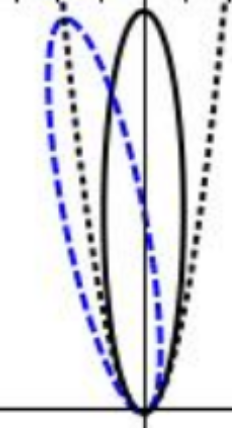
\includegraphics[scale=0.6]{orbits}
\caption{$r_{i}$ is the intersection of the two ellipses.}
\end{figure}

Let's be clear about what this means. The two ellipses are both defined by the equation $r(\phi)$.  The only difference between the two is the argument of the periapsis, $\phi_{p}$.  In order for the two ellipses to intersect, we require:

\begin{equation}
\frac{a(1 - \epsilon^2)}{1 + \epsilon \cos(\phi - \phi_{p})} = \frac{a(1 - \epsilon^2)}{1+\epsilon \cos(\phi - \phi_{p} - \delta \phi_{p})}
\end{equation}

But all this means is that $\cos(\phi - \phi_{p}) - \cos(\phi - \phi_{p} - \delta \phi_{p})$. This seems like it would be really ugly to solve, until we remember that $\cos(x)$ has some nice properties, specifically, that it is even and periodic.  Let $\phi = \delta \phi_{p} / 2$, and notice that we get

$$
\cos{(\delta \phi_{p}/2 - \phi_{p})} = \cos(-\phi_{p} - \delta \phi_{p} / 2) = \cos(\delta \phi_{p} / 2 - \phi_{p} - \delta \phi_{p}) 
$$

Now we can plug $\phi$ back into $r(\phi)$ and solve for $r_{i}$.  Doing so, we obtain:

\begin{equation}
r_{i} = \frac{r_{p} (1 + \epsilon)}{1 + \epsilon \cos(3 \pi M/ a(1 - \epsilon^2))}
\end{equation}
\end{alphaparts}

%==================== Question 12 ==================%
\question
The star known as S2 orbits the black hole at Sgr A* in the Galactic Center with a period of 15.9 yr.  The eccentricity of the orbit is $e = 0.8831 \pm 0.0034$ and the mass of the black hole $M_{\mathrm{bh}} = 4.30 \pm 0.27 \times 10^{6} M_{\odot}$.

\begin{alphaparts}
\questionpart
Estimate the relativistic precession of periapse angle per orbit.

Hartle (9.57) tells us that 
\begin{equation}
\delta \phi_{\mathrm{prec}} = \frac{6 \pi G}{c^2} \frac{M}{a (1 - \epsilon^2)}
\end{equation}
Note that we have the period.  To solve for the semimajor axis, $a$, we use Kepler and recover
$$ a = \big(\frac{T^2}{4\pi^2} GM \big)^{1/3} $$

Then we can evaluate these expressions.  Wolfram tells us that $a = 1.53 \times 10^{14} \mbox{ m}$. Thus, $\delta \phi = 0.0035 \mbox{ rad} = 0.2 \degree$. 

\questionpart
The latest estimate of the periapse angle is $\omega = 64.98\degree \pm 0.81 \degree$.  In view of the quoted $1 \sigma$ error, how long will it be before the precession is detected at $3\sigma$, assuming that the cadence and accuracy of the astrometric measurements remain constant?

We calculated the precession per orbit so we just want to see how many orbits it takes to go $2.4 \degree$ at $0.2 \degree$ per orbit.  The answer is 12.

\questionpart
Estimate the difference between the orbital period measured by astronomers -- defined as the time between periapses -- and that experienced by the proper time of S2 itself. 

This is analogous to problem 3.  We again use the Lorentz transform, setting $\bar{t} = \gamma(t - vx)$.  However, we have to solve for $x.$  $x$ is the circumference of the ellipse $2 \pi \sqrt{(a^2 + b^2)/2}$, where $b = a \sqrt{1 -e^2}$. Then we consider that $v = p/T$.  Therefore
$$
\bar{t} = \gamma (T - \frac{p^2}{T})
$$
\end{alphaparts}

%===================== Question 13 =================%
\question
In its equatorial plane ($\theta = \pi/2$), the metric of a rotating black hole reduces to
$$
ds^2 = - \Big(1 - \frac{2M}{r} \Big) dt^2 - \frac{4aM}{r}dtd\phi + \Big(r^2 + a^2 + \frac{2Ma^2}{r} \Big) d\phi^2 + \Big(1 - \frac{2M}{r} + \frac{a^2}{r^2} \Big)^{-1} dr^2
$$

\begin{alphaparts}
\questionpart
Find three constants of motion for timelike and null geodesics in the equatorial plane. 

For timelike geodesics $ds^2 < 0$, and for null geodesics $ds^2 = 0$.  We adopt an affine parameter $d\lambda = 1/m \cdot d\tau$. Then 
$$\frac{dx^{\mu}}{d\lambda} = \frac{dx^{\mu}}{d\tau} \frac{d\tau}{d\lambda} = u^{\mu}m = p^{\mu}$$.

Note that our metric does not have an explicit dependence on $t$ or $\phi$.  Therefore, there will be associated constants of motion.  Following the geodesic equation, we set $\alpha = t$ to find the first associated constant. 

$$g_{tt} \frac{dt}{d\lambda} + g_{t\phi} \frac{d\phi}{d\lambda} = E,$$ or explicitly
$$\Big(1 - \frac{2M}{r} \Big) \frac{dt}{d\lambda} +  \frac{2aM}{r} \frac{d\phi}{d\lambda} = E$$
Note that we have removed a factor of 2, because the $dtd\phi$ term in the metric included contributions from both $g_{t\phi}$ and $g_{\phi t}$.

Now set $\alpha = \phi$, and obtain
$$\frac{2aM}{r} \frac{dt}{d\lambda} + \Big(r^2 + a^2 + \frac{2aM}{r} \Big) \frac{d\phi}{d\lambda} = L $$

Our last constant of motion comes directly from the geodesic equation.  We divide through by $d\lambda^2$, noting that $(ds/d\lambda)^2 = p \cdot p = -m^2.$  This yields

$$
\centering
- \Big(1 - \frac{2M}{r} \Big) \Big(\frac{dt}{d\lambda}\Big)^2 - \frac{4aM}{r} \frac{dt}{d\lambda} \frac{d\phi}{d\lambda} + \Big(r^2 + a^2 + \frac{2Ma^2}{r} \Big) \Big( \frac{d\phi}{d\lambda} \Big)^2 +  \Big(1 - \frac{2M}{r} + \frac{a^2}{r^2} \Big)^{-1} \Big(\frac{dr}{d\lambda} \Big)^2 = -m^2 $$

\questionpart
Show that $g_{tt} g_{\phi \phi} - g_{t \phi}^2 = -r^2 (g_{rr})^{-1}$, and use this to solve for $dt/d\lambda$ and $d\phi / d\lambda$ in terms of (-E, L), where E and L are the constants of motion that reduce to $dt/d\lambda$ and to $r^2 d\phi / d\lambda$ as $r \to \infty$, respectively (i.e., the energy and angular momentum).

This is pretty much plug and chug.
\begin{subequations}
\begin{align*}
g_{tt}g_{\phi \phi} - g_{t \phi}^2 &= \Big(1 - \frac{2M}{r} \Big) \Big(r^2 + a^2 + \frac{2Ma^2}{r} \Big) + \Big(\frac{2aM}{r}\Big)^2 \\
&= r^2 + a^2 + \cancel{\frac{2ma^2}{r}} - 2Mr - \cancel{\frac{2ma^2}{r}} - \cancel{\frac{4M^2a^2}{r^2}} + \cancel{\frac{4M^2a^2}{r^2}} \\
&= r^2 + a^2 - 2Mr \\
&= -r^2 \Big(1 - \frac{2m}{r} + \frac{a^2}{r^2} \Big) \\
&= -\frac{r^2}{g_{rr}}
\end{align*}
\end{subequations}
Now we want to solve for $dt/d\lambda$ and $d\phi / d\lambda$.  From our definitions of $E$ and $L$ above, we can set
\begin{subequations}
\begin{align*}
\frac{dt}{d\lambda} &= \frac{1}{g_{tt}} \Big(E - g_{t\phi} \frac{d\phi}{d\lambda} \Big) \\
L &= g_{\phi \phi} \frac{d\phi}{d\lambda} + \frac{g_{t\phi}}{g_{tt}} \Big(E - g_{t \phi} \frac{d \phi}{d \lambda} \Big) \\
g_{tt} L - g_{t \phi} E &= \frac{d\phi}{d\lambda} \cancelto{\frac{-r^2}{g_{rr}}}{\Big(g_{\phi \phi}g_{tt} - g_{t \phi}^{2}\Big)}
\end{align*}
\end{subequations}
\begin{subequations}
\begin{align*}
\frac{d\phi}{d\lambda} &= - \frac{g_{rr}}{r^2} \Big(g_{tt}L - g_{t \phi} E\Big) \\
\frac{dt}{d\lambda} &= \frac{E}{g_{tt}} + \frac{g_{t \phi} g_{rr}}{r^2} \Big(g_{tt} - g_{t \phi}E \Big) 
\end{align*}
\end{subequations}

\questionpart
The horizon---the radius within which no future-directed timelike or null geodesic can escape to $r = \infty$---actually occurs not where $g_{tt} = 0$ but where $g_{rr} = \infty$.  Show that there are actually two roots $\{r_+, r_-\}$ for the horizon radius if $0 < \lvert a/M \rvert < 1$.  Show further that there is a radius $r_E$ such that there can be no timelike stationary observers [i.e., observers with $dr/d\tau = 0 = d\phi / d\tau$ in the region $\max(r_+, r_-) \leq r \leq r_E$], and express $r_E$ in terms of $a$ and $M$.  (This region is called the ergosphere).

Realize that $g_{rr} \to \infty$ when $1/g_{rr} \to 0$.  Then
$$\frac{1}{g_{rr}} = \Big(1 - \frac{2M}{r} + \frac{a^2}{r^2} \Big)$$  We multiply through by $r^2$ to obtain a quadratic.
$$ r^2 - 2Mr + a^2 = 0$$  This has two solutions, which are
$$ r_{\pm} = M \pm \sqrt{M^2 - a^2} $$ 

Now to find the limit for $r_E$ we set $dr/d\lambda = d\phi / d\lambda = 0$. which gives us

$$ -g_{tt} \Big(\frac{dt}{d\lambda}\Big)^2 = -m^2 $$

To obtain the limit of a timelike observer, the path has to be null, so $m^2 = 0$. Then $r_e$ is such that $g_{tt} = 0$, which occurs where $(1 - 2M/r) = 0$.  Therefore, $r_E = 2M$. 

\questionpart 
The horizon is generated by ``frozen'' null geodesics that neither fall into the black hole nor escape to $r = \infty$.  In these coordinates they are described by constant radii, $r = r_H \in \{r_+, r_-\}$, so that $dr / d\lambda = 0$ if $\lambda$ is an affine parameter.  Show that 
$$ \Omega_H = \Big(\frac{d\phi/d\lambda}{dt/d\lambda} \Big)_{r=r_H} $$ must be constant for such geodesics, and express $\Omega_H$ in terms of $a$, $M$, and $r_\pm$.  This is called the angular velocity of the horizon. 

When $r \in \{r_+, r_-\}$, we can see that it causes $L \to 0$.  Then we can see that 
$$ g_{\phi \phi} \frac{d\phi}{d\lambda} = -g_{\phi t} \frac{dt}{d\lambda} $$
$$ \Omega_H = \frac{2aM}{r_\pm} \Big(r_{\pm}^2 + a^2 + \frac{2ma^2}{r_{\pm}} \Big) $$
\end{alphaparts}

%======================= Question 14 =========================================

\question
It can be shown that in three dimensions, i.e., where the indices range from 0 to 2 (Lorentzian) or from 1 to 3 (Riemannian), the Riemann tensor can be expressed in terms of the Ricci tensor and Ricci scalar by 
\begin{equation}
R_{\lambda \mu \nu \kappa} = A(g_{\lambda \nu}R_{\mu \kappa} - g_{\lambda \kappa}R_{\mu \nu} - g_{\mu \nu}R_{\lambda \kappa} + g_{\mu \kappa} R_{\lambda \nu}) + BR(g_{\lambda \nu} g_{\mu \kappa} - g_{\lambda \kappa} g_{\mu \nu}),  
\end{equation}
where $R$ is the Ricci scalar (the trace of the Ricci tensor), for certain dimensionless constants $A$ and $B$.

\begin{alphaparts}
\questionpart
Determine A and B from the condition $g^{\lambda \nu} R_{\lambda \mu \nu \kappa} = R_{\mu \kappa}$.

Let's multiply through using the condition.  Doing so, we find
\begin{multline}
 g^{\lambda \nu} R_{\lambda \mu \nu \kappa} = A[ \cancel{\delta^{\lambda}_{\lambda} R_{\mu \kappa}} - \cancel{g_{\lambda \kappa} R_{\mu}^{\lambda}} - g_{\mu \nu}R_{\kappa}^{\nu} + g_{\mu \kappa} R] \\ 
 + B R [\delta_{\lambda}^{\lambda} g_{\mu \kappa} - g^{\lambda \nu} g_{\lambda \kappa} g_{\mu \nu}] = R_{\mu \kappa}
\end{multline}

$$
R_{\mu \kappa} = A[ - R_{\mu \kappa} + g_{\mu \kappa}R] + BR[g_{\mu \kappa} - g^{\lambda \nu}g_{\lambda \kappa}g_{\mu \nu} ]
$$

$(A+B)R g_{\mu \kappa} = 0$.  $A = -B$.  $A = -1$, $B = 1$.

\questionpart
Show that in 3D Einstein's equations imply that vacuum regions are locally flat.

Recall Einstein's equations, namely
\begin{equation}
R_{\mu \nu} - \frac{1}{2}R g_{\mu \nu} = 8 \pi G T_{\mu \nu}
\end{equation}
In vacuum, $T_{\mu \nu} = 0$. The trick here is that $R = R_{\lambda}^{\lambda} = g^{\lambda \kappa} R_{\kappa \lambda}$.  Then we can write $Rg_{\mu \nu} = g^{\nu \mu}R_{\mu \nu}g_{\mu \nu}$.  Note that we can move around the sums, and that $g^{\nu \mu} g_{\mu \nu} = 1$. This lets us say 
$$ R_{\mu \nu} = \frac{1}{2} R_{\mu \nu} $$ which clearly implies $R_{\mu \nu} = 0$. 
\end{alphaparts}

%===================== Question 15 ===================================

\question
An astronaut finds herself in free fall in outer space, and not rotating.  She is equipped with some small useless objects, and to combat boredom while she awaits rescue, she flings these away from herself.  Regardless of the magnitude or direction of the initial velocity she imparts to them, the objects return to her after about one hour with minus their initial velocity, each along the same line as that by which it left her.

\begin{alphaparts}
\questionpart
She deduces that the space around her, although transparent and offering no resistance, is not a true vacuum.  Why not?

Spacetime curvature is detected via tidal forces.  These forces are specified by the tidal tensor, $\mathcal{T}$.  $$\mathcal{T}_{\hat{i}\hat{j}} = - \frac{\partial^2 \Phi}{\partial x^i \partial x^j} $$ We should also note that $\mathrm{Tr}(\mathcal{T}) = \nabla^2 \Phi = 4 \pi G \rho$.

If the ball comes back from any direction, then all three directions ($i, j, k$) have a negative tidal field.  The fact that the motion is isotropic implies a harmonic oscillator.  Then $\mathcal{T}_{\hat{i} \hat{j}} = -\omega^2 \delta_{\hat{i} \hat{j}}$, and $\omega = 2\pi / T$.  The fact that there are tidal forces implies that $\rho \neq 0$, which means we are not in a vacuum. 

\questionpart
Estimate the local matter density in $\mbox{ g}\mbox{ cm}^{-3}$, not including the contribution of her own body. 

We take the trace, and note that the period of oscillation is two hours.  Then we can solve.
$$\mathrm{Tr}(\mathcal{T}) = 3 \omega^2 = 4 \pi G \rho$$

$$\rho = \frac{3 \omega^2}{4 \pi G} = \frac{3 \pi}{G} \cdot \frac{1}{(2 \cdot 3600)^2} $$

Which yields
$\rho \approx 2725 \mbox{ kg} \mbox{ m}^{-3}$.

\end{alphaparts}

%==================== Question 16 ==================================
\question
Consider cosmological perfect fluid with $p = w \rho$ where $w$ is a constant factor.  Assume the universe is spatially homogeneous and isotropic and that the fluid is comoving, i.e., its energy-momentum tensor is $T^{\hat{0}\hat{0}} = \rho$, $T^{\hat{i}\hat{j}} = \rho \eta^{\hat{i}\hat{j}}$ in an orthonormal basis based on the usual cosmological coordinates $t r \theta \phi$. 

\begin{alphaparts}

\questionpart
Show that $\rho \propto a^q$ as the scale factor $a$ in the cosmological metric changes with time, and relate the exponent $q$ to $w$. 

For a perfect fluid, $T^{\mu \nu} = (\rho + p) U^{\mu} U^{\nu} + p g^{\mu \mu}$, (lecture 15 slides).  In the orthonormal basis, $T^{\mu \nu} = \mathrm{diag}(\rho, P, P, P)$.  Conservation of energy and momentum tells us that $T_{; \nu}^{\mu \nu} = 0$.  The lecture 17 slides tell us that

$$T_{; \nu}^{0 \nu} = \dot{\rho} - 3a\dot{a} \frac{p}{a^2} + \frac{3\dot{a}}{a} \rho = 0$$

$$\dot{\rho} + \frac{3\dot{a}}{a} \rho = \frac{3 \dot{a}}{a} p $$

Which is the same (?) as the first law of thermodynamics for cosmology, namely that 
\begin{equation}
\frac{d}{dt}[ \rho(t) a^3(t)] = -p \frac{d}{dt} [a^3(t)] 
\end{equation}

Then letting $p = w \rho$, that gives us

$$\dot{\rho} + \frac{3\dot{a}}{a}(1 + w) \rho = 0$$

Yielding

$$\frac{\dot{\rho}}{\rho} = -3(1 + w)\frac{\dot{a}}{a} \to \rho \propto a^{-3(1+w)} $$

Although I am a little uncertain about this derivation it is in the lecture 17 slides and you can hopefully just copy those down on the final.

\questionpart
Suppose $q = -1$.  (This could be approximated, for example, by a ``foam'' of domain walls consisting of false vacuum---and unlikely model for the present universe.  Such walls would have constant surface tension $\kappa$ and mass per unit area $\sigma$ related by $\sigma = -\kappa >0.$) Supposing that this fluid makes the only significant contribution to the mass and energy density, discuss the evolution of $a(t)$ for universes of positive, negative, and zero spatial curvature.  In which cases can there be a ``big bang,'' i.e., $a$ starting from zero?  In which cases can $\dot{a}$ change sign? 

Whenever we want to find the evolution of $a$, we use the Friedmann Equation 
\begin{equation}
\Big(\frac{\dot{a}}{a}\Big)^2 + \frac{k}{a^2} = \frac{8 \pi G \rho}{3}
\end{equation}

Because $q = -1$ that implies $\rho = \rho_0 a_0 / a$. Then, substituting for $\rho$ and multiplying through by $a^2$, we have

$$\dot{a}^2 + k = Qa$$

where $Q = 8 \pi G \rho_0 a_0 / 3$ and is a constant.  This yields a quadrature for $a(t)$, the integration of which is pretty trivial.

$$ \frac{da}{\sqrt{Qa - k}} = \pm dt \to \frac{2}{Q}\sqrt{Qa - k} = \pm t$$

The sign of $\dot{a}$ can change in a closed universe which is when $k>0$.  We can only have $a=0$ if $k \leq 0$.  The discrepancy between this universe and the one in problem 17 is that this one is a fluid, whereas the one in 17 is radiation.
\end{alphaparts}

%========================== Question 17 ================================
\question 
\color{red}
Take this solution with a grain of salt... I'm unsure about my answer to the ODE, but I think the principle is more or less correct. \\ \\
\color{black}
Consider a positively curved universe consisting of pure radiation (i.e. $\Omega_m = \Omega_\lambda = 0, p = \rho/3$). For convenience, scale the comoving coordinates so that $k = 1$, i.e.

$$ ds^2 = -dt^2 + a^2(t) [d\chi^2 + \sin^2 \chi (d\theta^2 + \sin^2 \theta d\phi^2)]$$

A noninteracting massless particle is emitted from $\chi = 0$ at $t = 0$ (the Big Bang) and follows a radial null geodesic.  How far does it travel (maximum $\chi$) before the Big Crunch (the time at which $a(t)$ returns to zero)?

The fact that we have a radial null geodesic gives us $ds^2 = d\theta^2 = d\phi^2 = 0$. This gives us a simpler equation of motion:

$$-dt^2 + a^2(t) d\chi^2 = 0$$

Which we can move around to get a quadrature for $\chi(t)$

$$d\chi = \pm \frac{dt}{a(t)}$$

What does the $\pm$ mean?  It means that we can look at either the positive ($t>0$) or negative ($t<0$) null light cones.  We are only concerned with the positive case, as that is what corresponds to the universe.  To get further we have to find $a(t)$ explicitly.  We approach this, as in problem 16, via the Friedmann equation.  In the radiation only case, however, we have $\rho = \rho_{\mathrm{crit}} \Omega_r / a^4 = \rho_r / a^4$.  What makes our solution a little sketchy is the presence of $k$.  Substituting into the Friedmann equation and multiplying through by $a^2$, we have 

$$
\dot{a}^2 = \frac{Q}{a^2} - 1
$$

Which Wolfram tells us yields
$$
a(t) = \pm \sqrt{Q - t^2}
$$

Now we can go back and solve for $\chi(t)$.  Recall that the critical values of a function occur when the derivative is 0 or does not exist.  We get 

$$
d\chi = \frac{dt}{\sqrt{Q - t^2}}
$$
Which suggests that $t_{\chi_{\mathrm{max}}} = \sqrt{Q}$.  Then to obtain the total path length we solve for $\chi_{\mathrm{max}}$ and double it.

\setcounter{questionCounter}{0}

\subsection*{2013 Final Exam Answers}

%======================== Question 1 ==========================
\question
Consider the process $\gamma + e^- \to e^- + e^+ + e^-$ in a frame where the initial electron is at rest.  What is the minimum energy ($E_\gamma$) of the photon such that this process is possible?  Express your answer in terms of the electron rest mass, $m_e$.

We can approach this question using the respective four-momenta.  Consider that

$$p_{i}^2 = p_{f}^2 $$

Because we are finding the minimal energy, all of the products are also at rest.  With the initial electron at rest, the only thing not at rest is the photon.  Then we can write out the momentum four-vectors (in $c=1$ units).

\begin{subequations}
\begin{align*}
p_\gamma &= (E_\gamma, E_\gamma, 0, 0) \\
p_{e^-} &= (m_e, 0, 0, 0) \\
p_f &= (3m_e, 0, 0, 0) \\
p_i &= p_\gamma + p_{e^-} = (E_\gamma + m_e, E_\gamma, 0, 0)
\end{align*}
\end{subequations}

Now we set $p_{i}^2 = p_{f}^2$, remembering that we use the appropriate 4-vector dot product.

\begin{subequations}
\begin{align*}
-(E_\gamma + m_e)^2 + E_\gamma^2 &= -9m_e^2 \\
\cancel{-E_\gamma^2} + \cancel{E_\gamma^2} - 2m_e E_\gamma - m_e^2 &= -9m_e^2 \\
E_\gamma &= 4m_e
\end{align*}
\end{subequations}

\color{red}
Questions 2 and 3 are already on the review sheet as questions 2 and 7
\color{black}
\setcounter{questionCounter}{3}

\question
A nonrotating neutron star of mass $M = 1.5 M_{\odot}$ has radius $R = 9$ km (i.e., this is its circumference divided by $2 \pi$.  In answering the following questions, take $2GM_{\odot}/c^2 = 3$ km to simplify the arithmetic.

\begin{alphaparts}
\questionpart
A hydrogenic iron atom resting on the stellar surface undergoes a transition from the $n=2$ to $n=1$ state, releasing a photon with energy $6.7$ keV in its local frame.  What energy do astronomers (stationary observers at $r \gg 2M$) measure for this photon?

The photon is gravitationally redshifted because it loses energy climbing out of the potential well.  For this case, we realize that

$$E_{obs} \sqrt{1 - \frac{R_s}{r_{obs}}} = E_{em} \sqrt{1 - \frac{R_s}{r_{em}}} $$

Where we take $r_{obs} \to \infty$ and therefore

$$E_{obs} = E_{em} \sqrt{1 - \frac{R_s}{r_{em}}} $$

We can also solve this using the principle of equivalence for gravitational redshift.  Recall that

\begin{equation}
\nu_{a} \approx \nu_{b} \Big(1 + \frac{\Phi{b} - \Phi{a}}{c^2} \Big)
\end{equation}
where $\Phi_{a,b} = -GM/r$.  We also recall $E = h\nu$.  Then we can say
\begin{subequations}
\begin{align*}
h\nu_{a} &= h\nu_{b} \Big(1 + \frac{\frac{-G(1.5M_{\odot})}{9 \mbox{ km}}}{c^2} \Big) \\
&= h \nu_{b} \Big(\frac{3}{4}\Big) \\
&\approx 5 \mbox{ keV}
\end{align*}
\end{subequations}

\questionpart
An ``atmosphere'' of hydrogen 1 meter thick sits atop the surface at 9 km.  What is $r$ at the top of the atmosphere? 

We can compute the redshift $z$ by noting that $1 + z = \nu_{e} / \nu_{o}$.  Furthermore, $\gamma = 1 + z$.  So $\gamma = 4/3$. Then we contract the 1 meter atmosphere by dividing by $\gamma$ and get that it has a height of $0.75 \mbox{ m}$.  

\questionpart
Show that the astronomers can ``see'' (i.e., receive photons from) more than a hemisphere.

From Gauss' theorem, we can treat the neutron star as a point mass at $r=0$.  The source of the light is at $r = 9 \mbox{ km}$.  We can use the gravitational lensing equation to compute the deflection angle $\Delta \phi$.

$$\Delta \phi = \frac{2r_s}{r}$$ 

Then we solve for $\Delta \phi$ and see that it is non-zero.

\questionpart
What is the radius needed for a creature on the planet of the neutron star to see its own head?  Compare to the radius needed for astronomers to see the entire surface of the star.

For the creature to see its own head, $\Delta \phi = 2\pi$.  For astronomers to see the surface, $\Delta \phi = \pi$.

\end{alphaparts}

%============================ Question 5 ====================================
\question
De Sitter space is a cosmological model devoid of matter and radiation ($\Omega_{m} = \Omega_{r} = 0$), but with positive curvature and cosmological constant: $\Lambda, k > 0$. 


\begin{alphaparts}
\questionpart
What is the line element for this cosmology?

The line element is the one from the closed universe (i.e.)
\begin{equation}
ds^2 = -dt^2 + a^2(t)(d \chi^2 + sin^2 (\chi) d\Omega^2)
\end{equation}

\questionpart
Solve the Friedman equation for the evolution of the scale factor.  Show that it has non-zero minimum value.

Again we use the Friedman equation.  Evaluating with $\Omega_{m} = \Omega_{r} = 0$ gives us
the specific one for this problem.

$$
\Big( \frac{\dot{a}}{a} \Big)^2 = \frac{8 \pi G \rho a^2}{3} - k
$$

Which we can reduce to quadrature, yielding

$$
\frac{da}{\sqrt{(Q - \Lambda/3)a^2 - k}} = dt
$$
To solve this integral, factor the integrand denominator to get something in your integral table.  We can see from the form of the denominator that there is a minimum value for $a$, because the argument cannot be less than 0.

\questionpart
Can comoving observers always send and receive signals to each other? 

No.  The expansion eventually proceeds at greater than c, which means they can't.  In the limit of large time, our universe may approach a de Sitter universe.

\end{alphaparts}
\end{document}